\documentclass[9pt, handout]{beamer}
\usetheme{CambridgeUS}
\usepackage{xcolor}
\usepackage{geometry}
\usepackage{array}
\usepackage{comment}
\usepackage[export]{adjustbox}

\AtBeginSection[]
{
  \begin{frame}
    \frametitle{Table of Contents}
    \tableofcontents[currentsection]
  \end{frame}
}

\setbeamertemplate{footline}
{
  \leavevmode%
  \hbox{%
    \begin{beamercolorbox}[wd=.333333\paperwidth,ht=2.25ex,dp=1ex,center]{author in head/foot}%
      \usebeamerfont{author in head/foot}\insertshortauthor
    \end{beamercolorbox}%
    \begin{beamercolorbox}[wd=.333333\paperwidth,ht=2.25ex,dp=1ex,center]{title in head/foot}%
      \usebeamerfont{title in head/foot}\insertshortsubtitle
    \end{beamercolorbox}%
    \begin{beamercolorbox}[wd=.333333\paperwidth,ht=2.25ex,dp=1ex,right]{date in head/foot}%
      \usebeamerfont{date in head/foot}\insertshortdate{}\hspace*{2em}
      \usebeamertemplate{page number in head/foot}\hspace*{2ex}
    \end{beamercolorbox}
  }%
  \vskip0pt%
}

\title{Principles of Economics}
\subtitle{Discussion Session 6: Entry and Exit Decisions}
\author{Joe Wilske and Yuzhi Yao}
\institute{Boston College}
\date{\today}

\begin{document}

\frame{\titlepage}

\begin{frame}{Exercise 1: Profit Maximization}
    Q1: Suppose Amelia's Taqueria operates in a competitive market and maximizes its profits. If the market price is $P7$, which quantity level should the firm choose? Find regions representing \textbf{total revenue}, \textbf{total cost}, \textbf{variable cost}, and \textbf{profit}. 
    \begin{figure}
        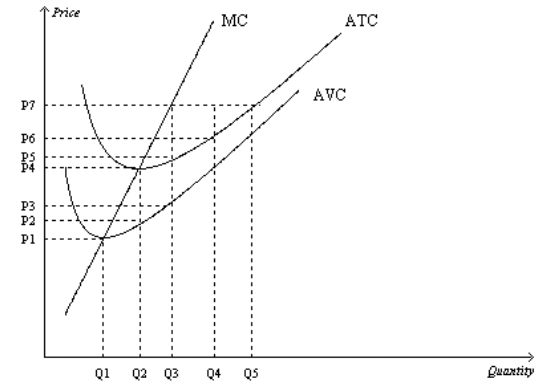
\includegraphics[width=0.6\textwidth, left]{fig1.png}
    \end{figure}
\end{frame}

\begin{frame}{Exercise 1: Profit Maximization}
    Solution: 
    \begin{itemize}
        \item[-] Profit-maximizing quantity is $Q3$ ($P=MR=MC$)
        \item[-] $TR =P7\times Q3$
        \item[-] $TC =P5\times Q3$
        \item[-] $VC =P3\times Q3$
        \item[-] $Profit = (P7-P5)\times Q3$
    \end{itemize}
    \vspace{1.5in}
\end{frame}

\begin{frame}{Exercise 2: Shut Down in Short-Run vs Long-Run}
    Q2: Should Amelia shut down her taqueria in the short run if the market price is P7? P3? Below P1? How about in the long run?
    \vspace{0.1in}
    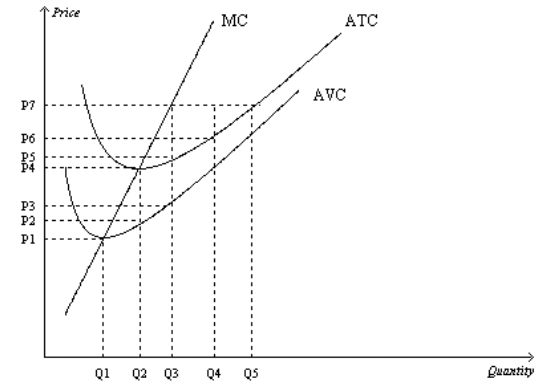
\includegraphics[width=0.6\textwidth, left]{fig1.png}
\end{frame}

\begin{frame}{Exercise 2: Shut Down in Short-Run vs Long-Run}
    Solution: 
    \vspace{10pt}
    \begin{itemize}
        \item[-] When price is $P7$: Making positive profits :) \\
        $\implies$ Keep operating in both short- and long-run.
        \vspace{10pt}
        \item[-] When price is $P3$: Making losses, but the firm can cover its variable costs and part of its fixed costs. \\
        $\implies$ Operate in short-run but shut down in long-run.
        \vspace{10pt}
        \item[-] When price is below $P1$: Making losses, and can't even cover variable costs :(\\
        $\implies$ Shut down immediately.
    \end{itemize}
    \vspace{1.5in}
\end{frame}

\begin{frame}{Summary: Shut Down in Short-Run vs Long-Run}
    \begin{table}[]
    \centering
    \begin{tabular}{lll}
    \hline
    Situation & Profit = TR - TC & Decision \\
    \hline
    Price $>$ ATC & Positive & Keep operating in short- and long-run \\
    AVC $<$ Price $<$ ATC & Negative & Keep operating in short-  \\
     & & but shut down in long-run \\
    Price $<$ AVC & Negative & shut down in short- and long-run \\
    \hline
    \end{tabular}
\end{table}
    \vspace{1.5in}
\end{frame}

\begin{frame}{Effect of Entry and Exit on Aggregate Supply}
    Suppose there is a negative demand shock in the market for Mexican food.
    \begin{itemize}
        \item Demand curve shifts left.
        \item Price falls from $P_4$ to $P_3$.
    \end{itemize}
    \begin{enumerate}
        \item How will this effect Mexican restaurants' profits? How will they react?
        \item What will happen to the aggregate supply curve over time?
    \end{enumerate}
    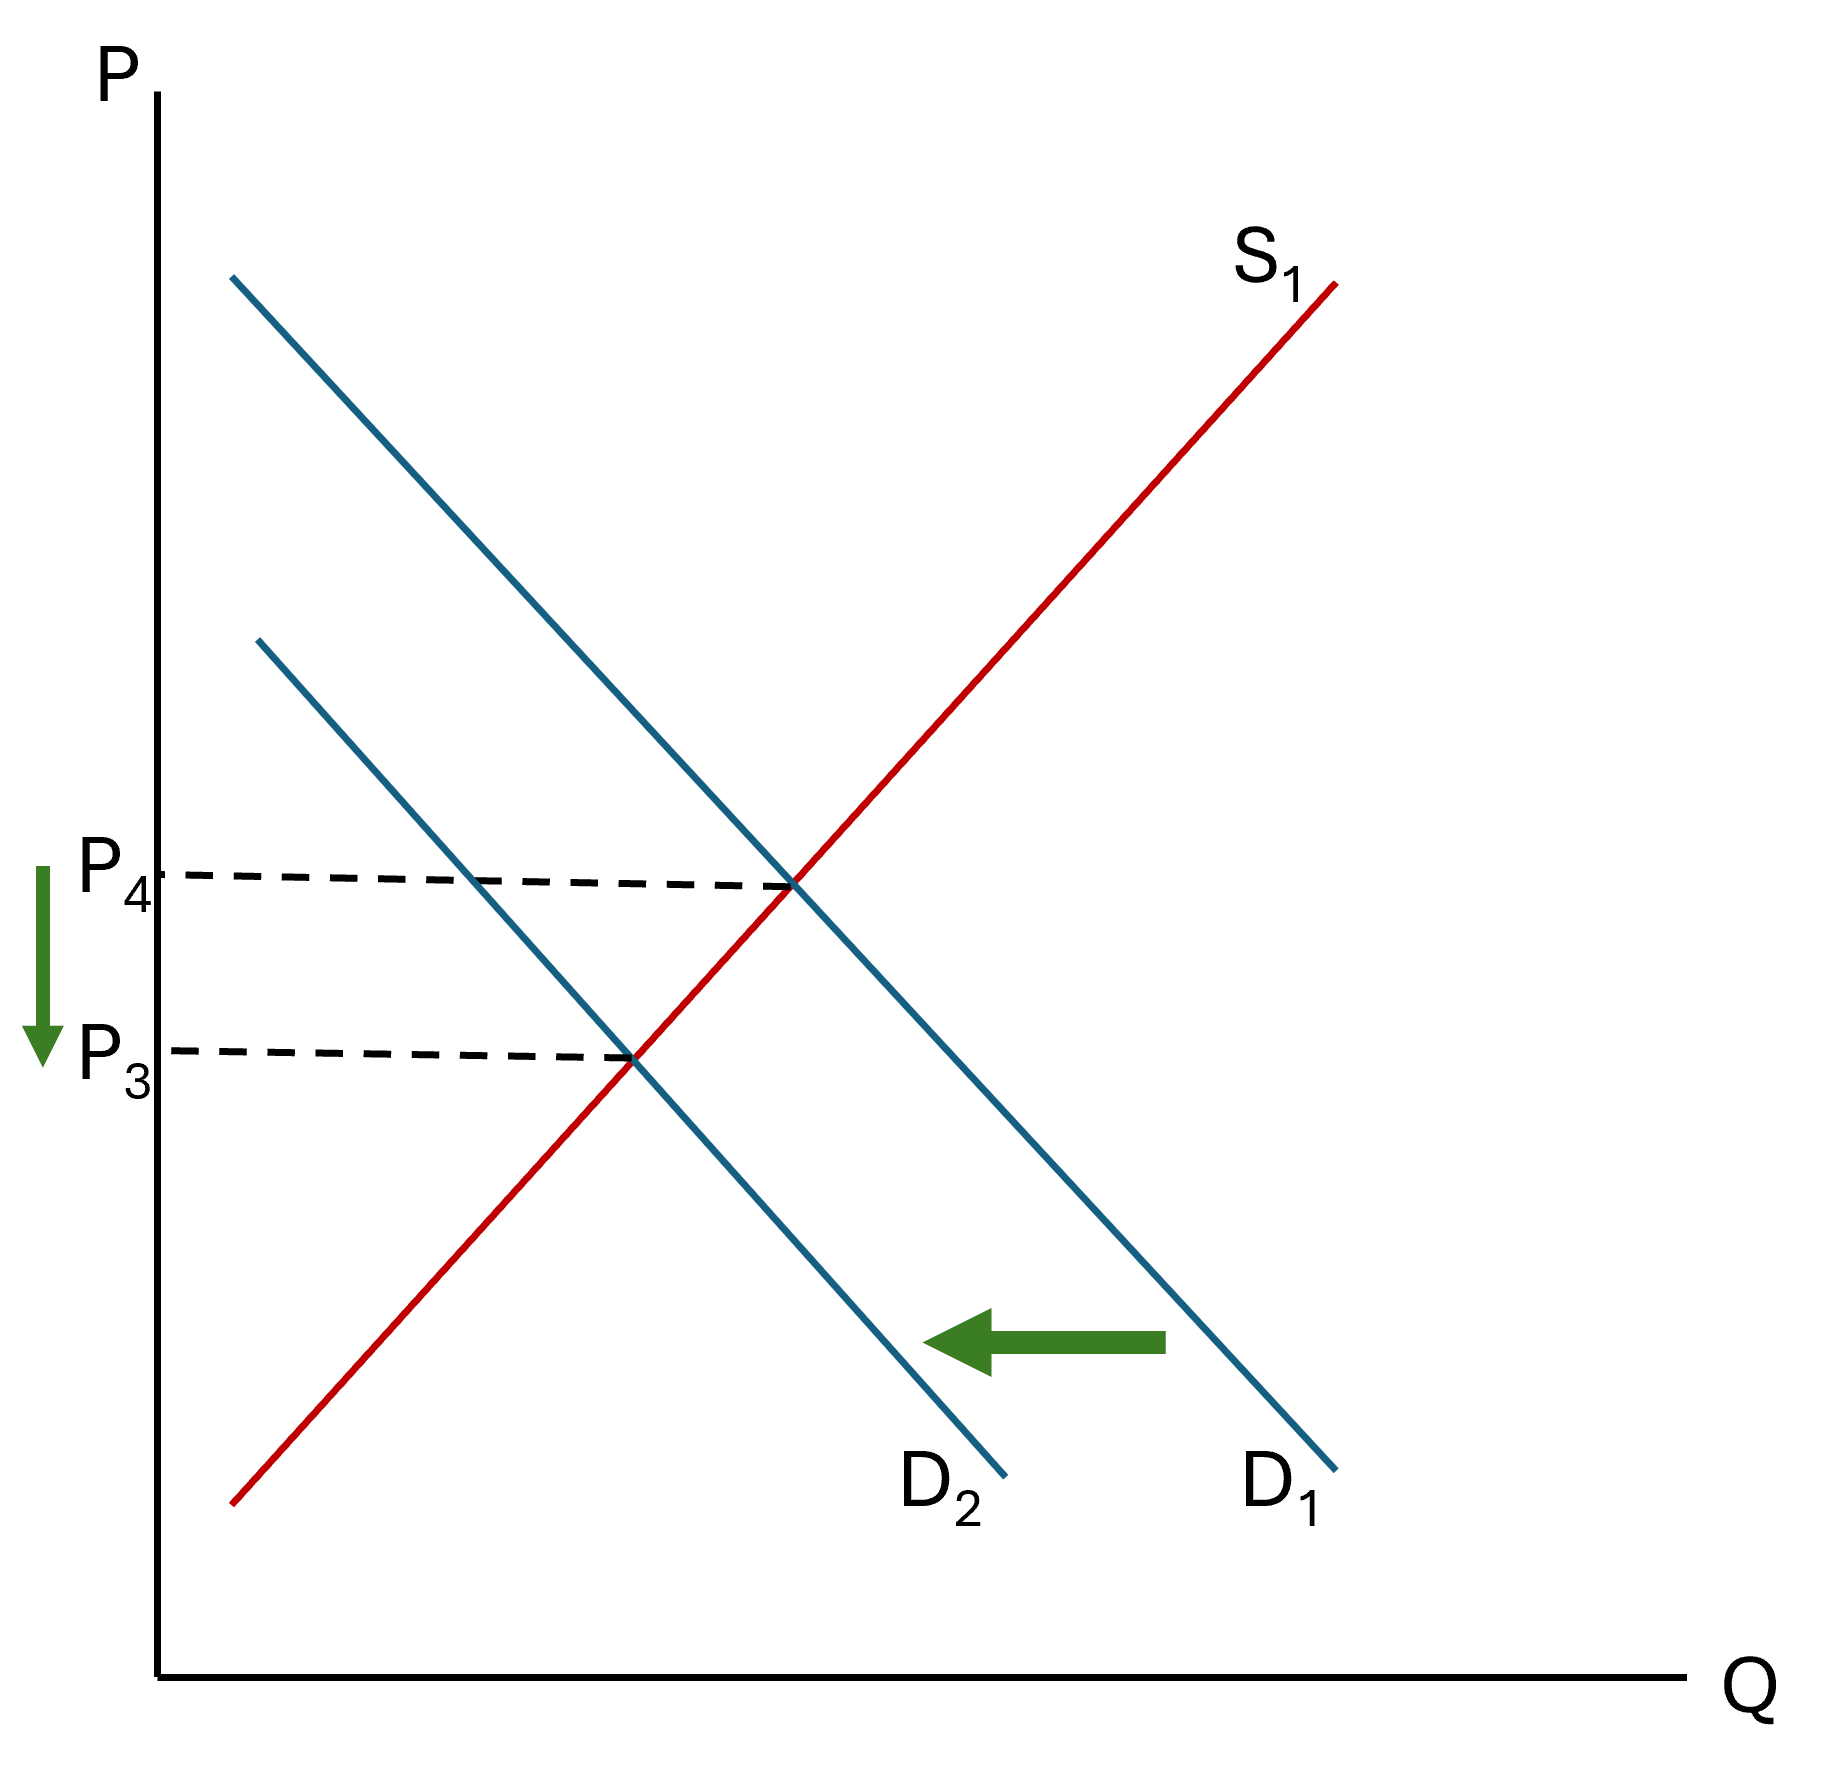
\includegraphics[width=.5\linewidth]{demand_falls.png}
\end{frame}

\begin{frame}{Effect of Entry and Exit on Aggregate Supply}
    Suppose there is a negative demand shock in the market for Mexican food.
    \begin{enumerate}
        \item How will this effect Mexican restaurants' profits? How will they react?\\
        $\implies$ Negative profits cause long-run exits.
        \item What will happen to the aggregate supply curve over time?\\
        $\implies$ Aggregate supply shifts left as restaurants exit, until $P$ returns to $P_4$.
    \end{enumerate}
    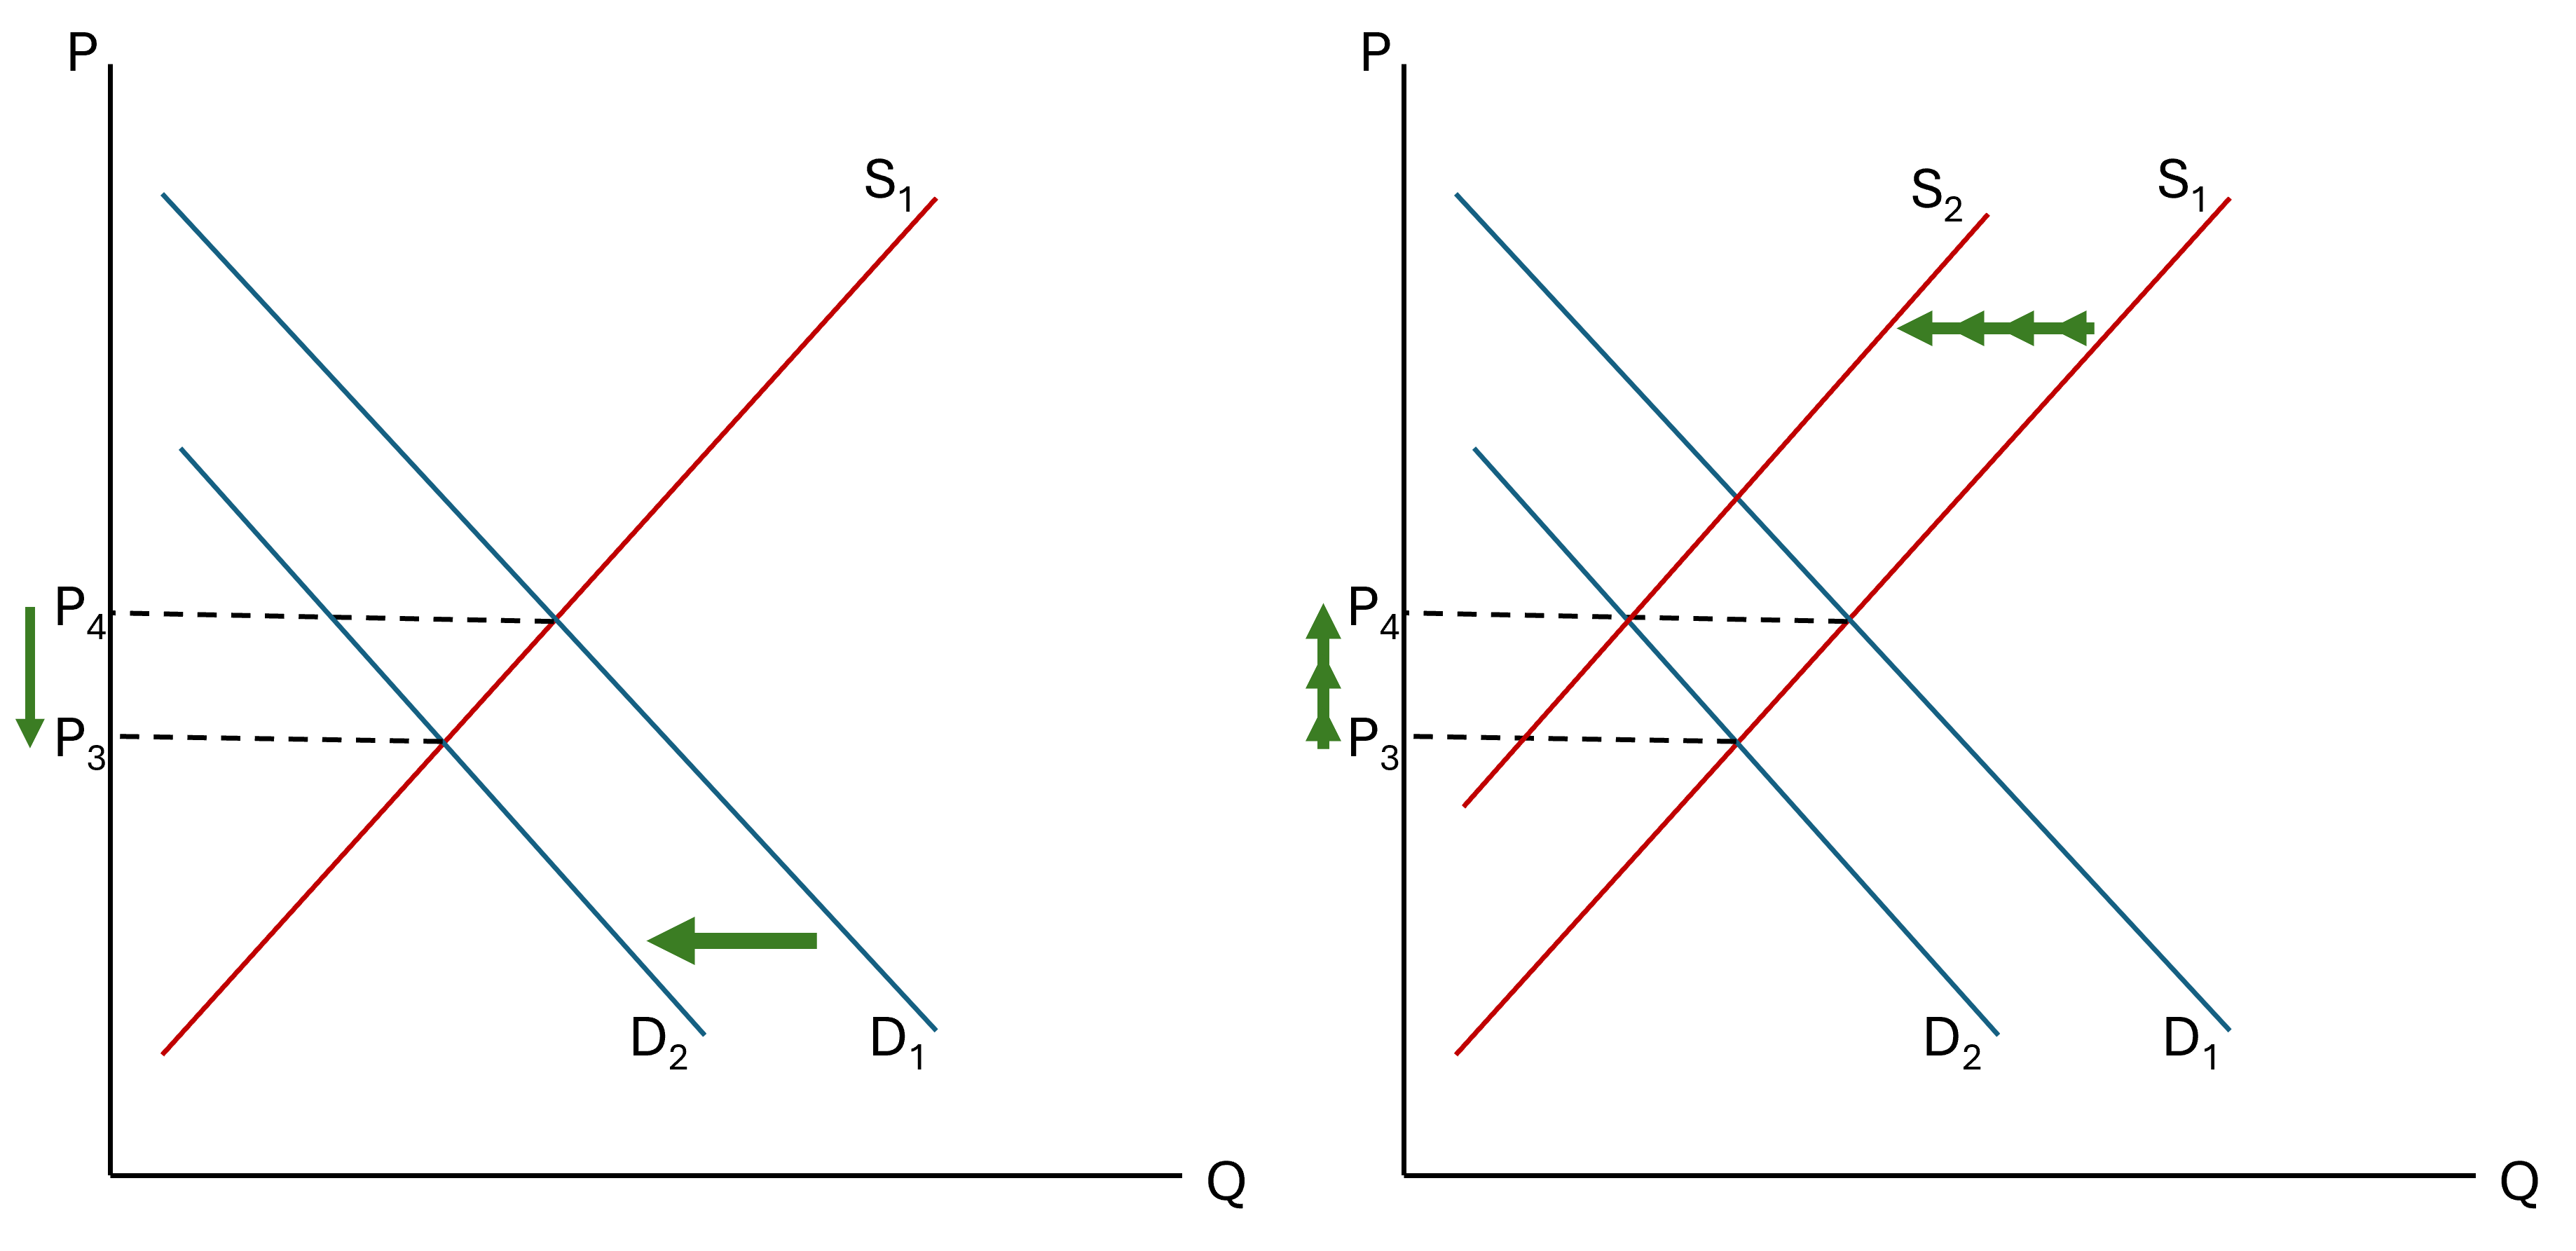
\includegraphics[width=\linewidth]{supply_falls.png}
\end{frame}

\begin{frame}{Exercise 3: Supply in Short-Run vs Long-Run}
    Suppose Mexican food suddenly becomes popular in Boston.
    \begin{itemize}
        \item Demand curve shift right.
        \item Equilibrium price increases from $P_4$ to $P_7$.
    \end{itemize}
    \begin{enumerate}
        \item How will this effect Mexican restaurants' profits? How will they react?
        \item What will happen to the aggregate supply curve over time?
        \item How will the equilibrium price change over time?
    \end{enumerate}
    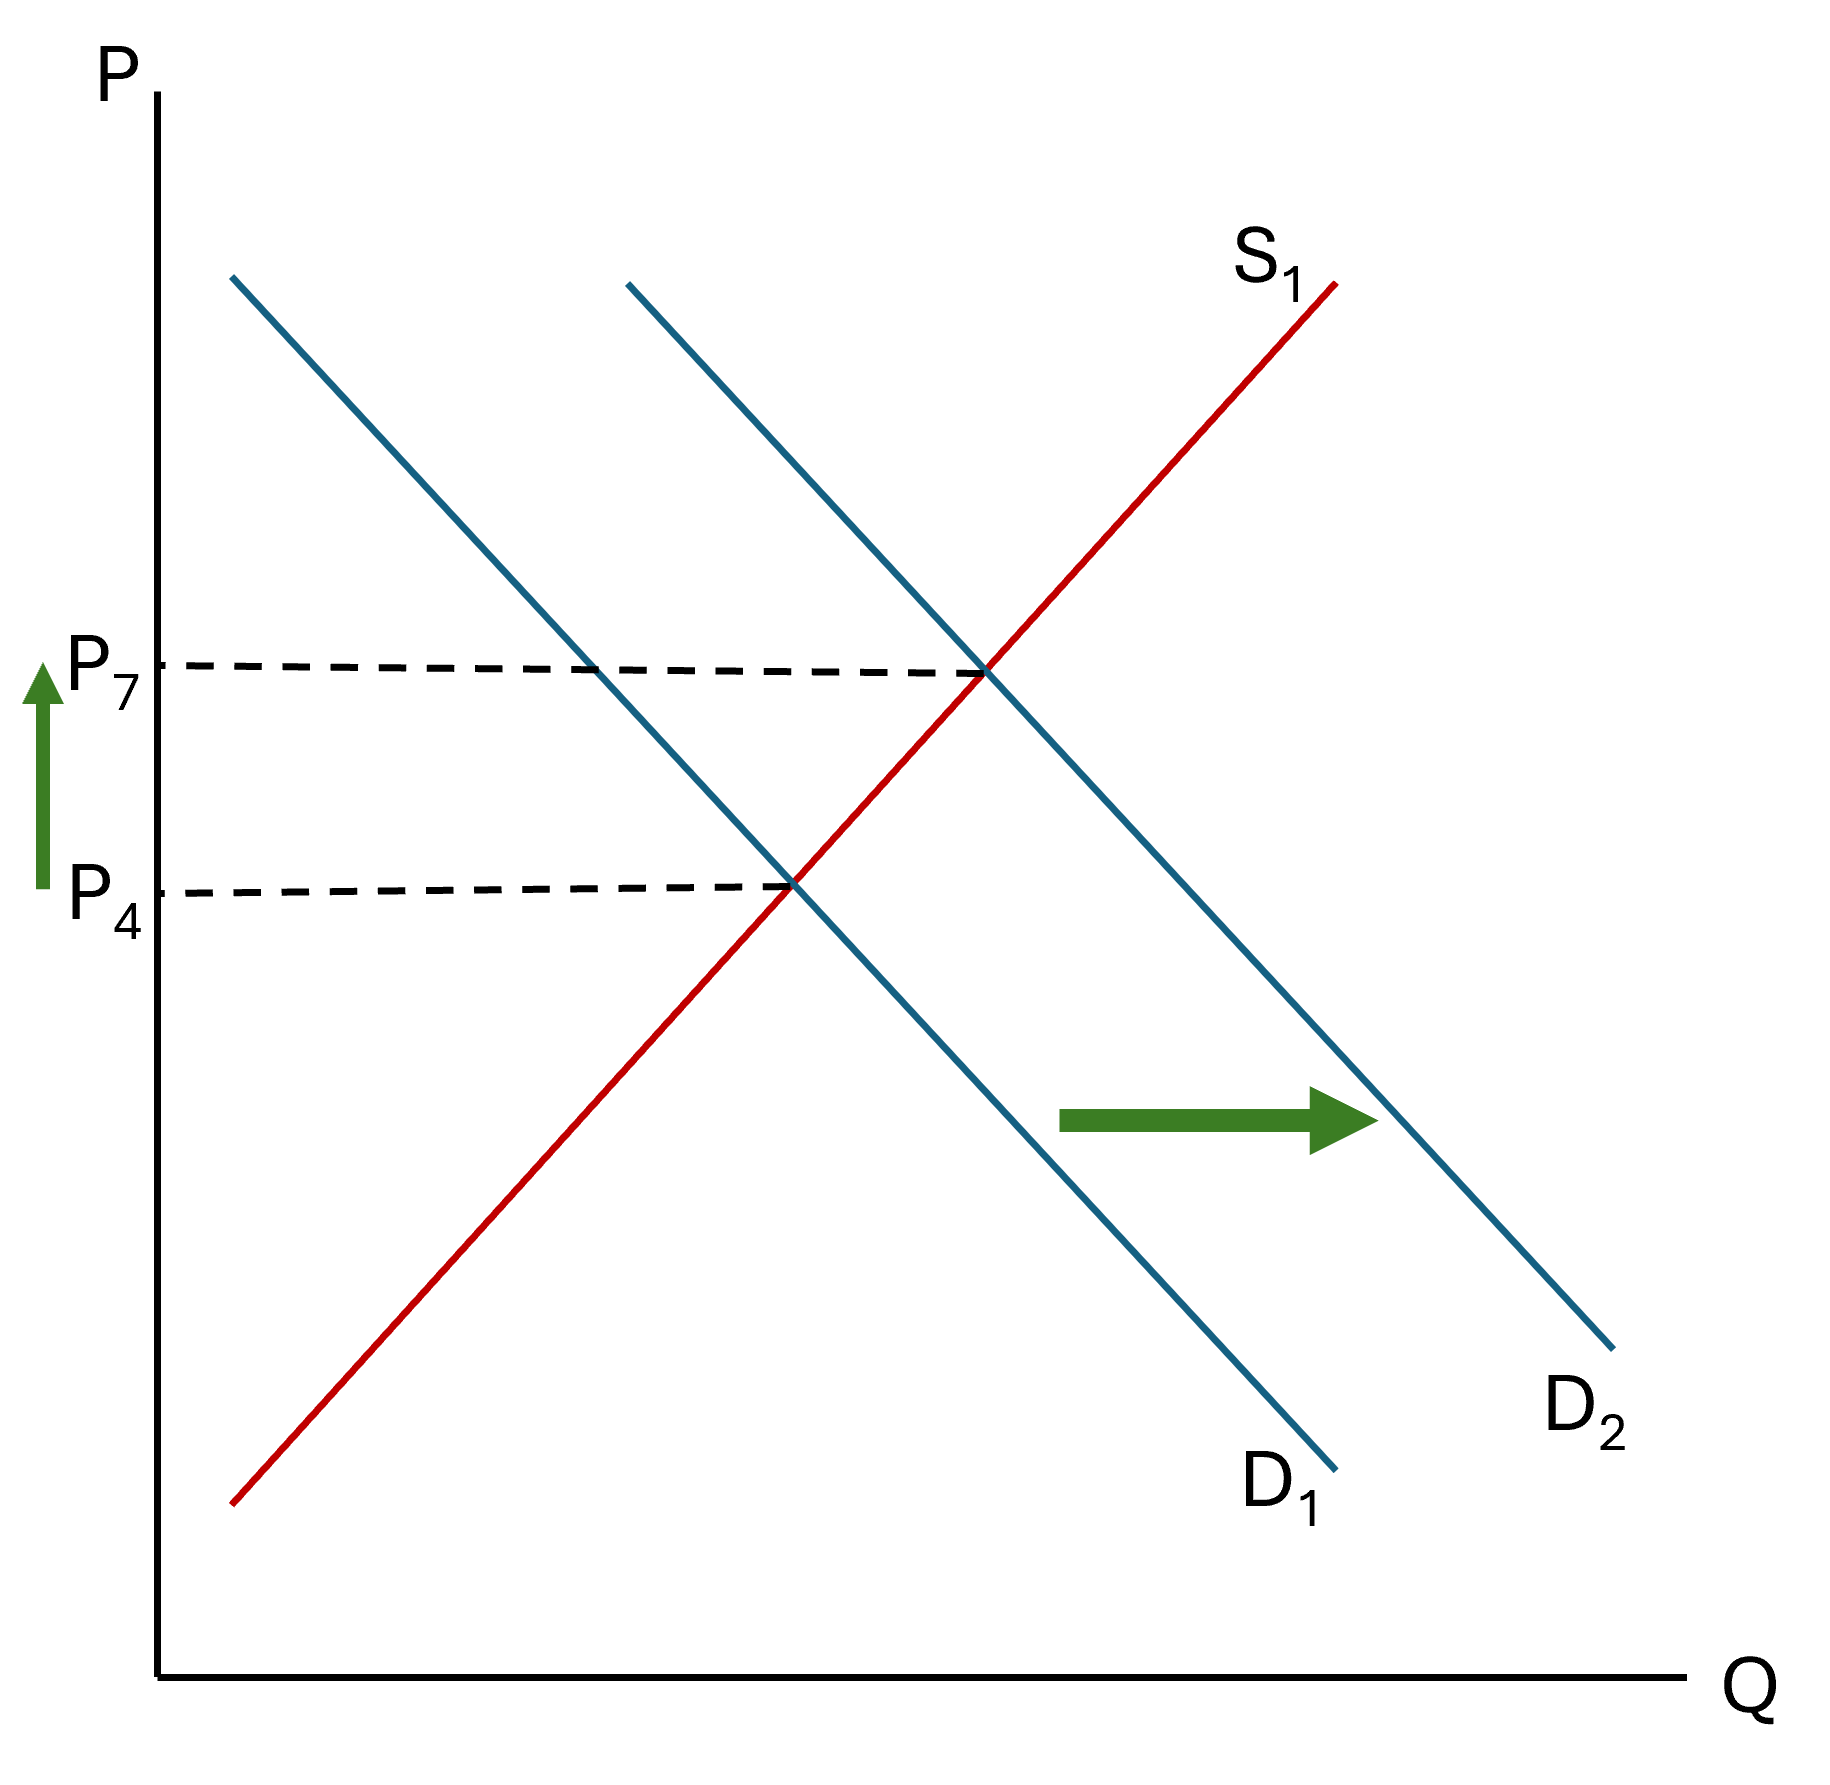
\includegraphics[width=.4\linewidth]{demand_increases.png}
\end{frame}

\begin{frame}{Exercise 3: Supply in Short-Run vs Long-Run}
    Solution:
    \begin{enumerate}
        \item Positive profits cause new entries.
        \item Aggregate supply shifts to the right.
        \item Supply increases until $P$ returns to $P_4$ and entries cease.
    \end{enumerate}
    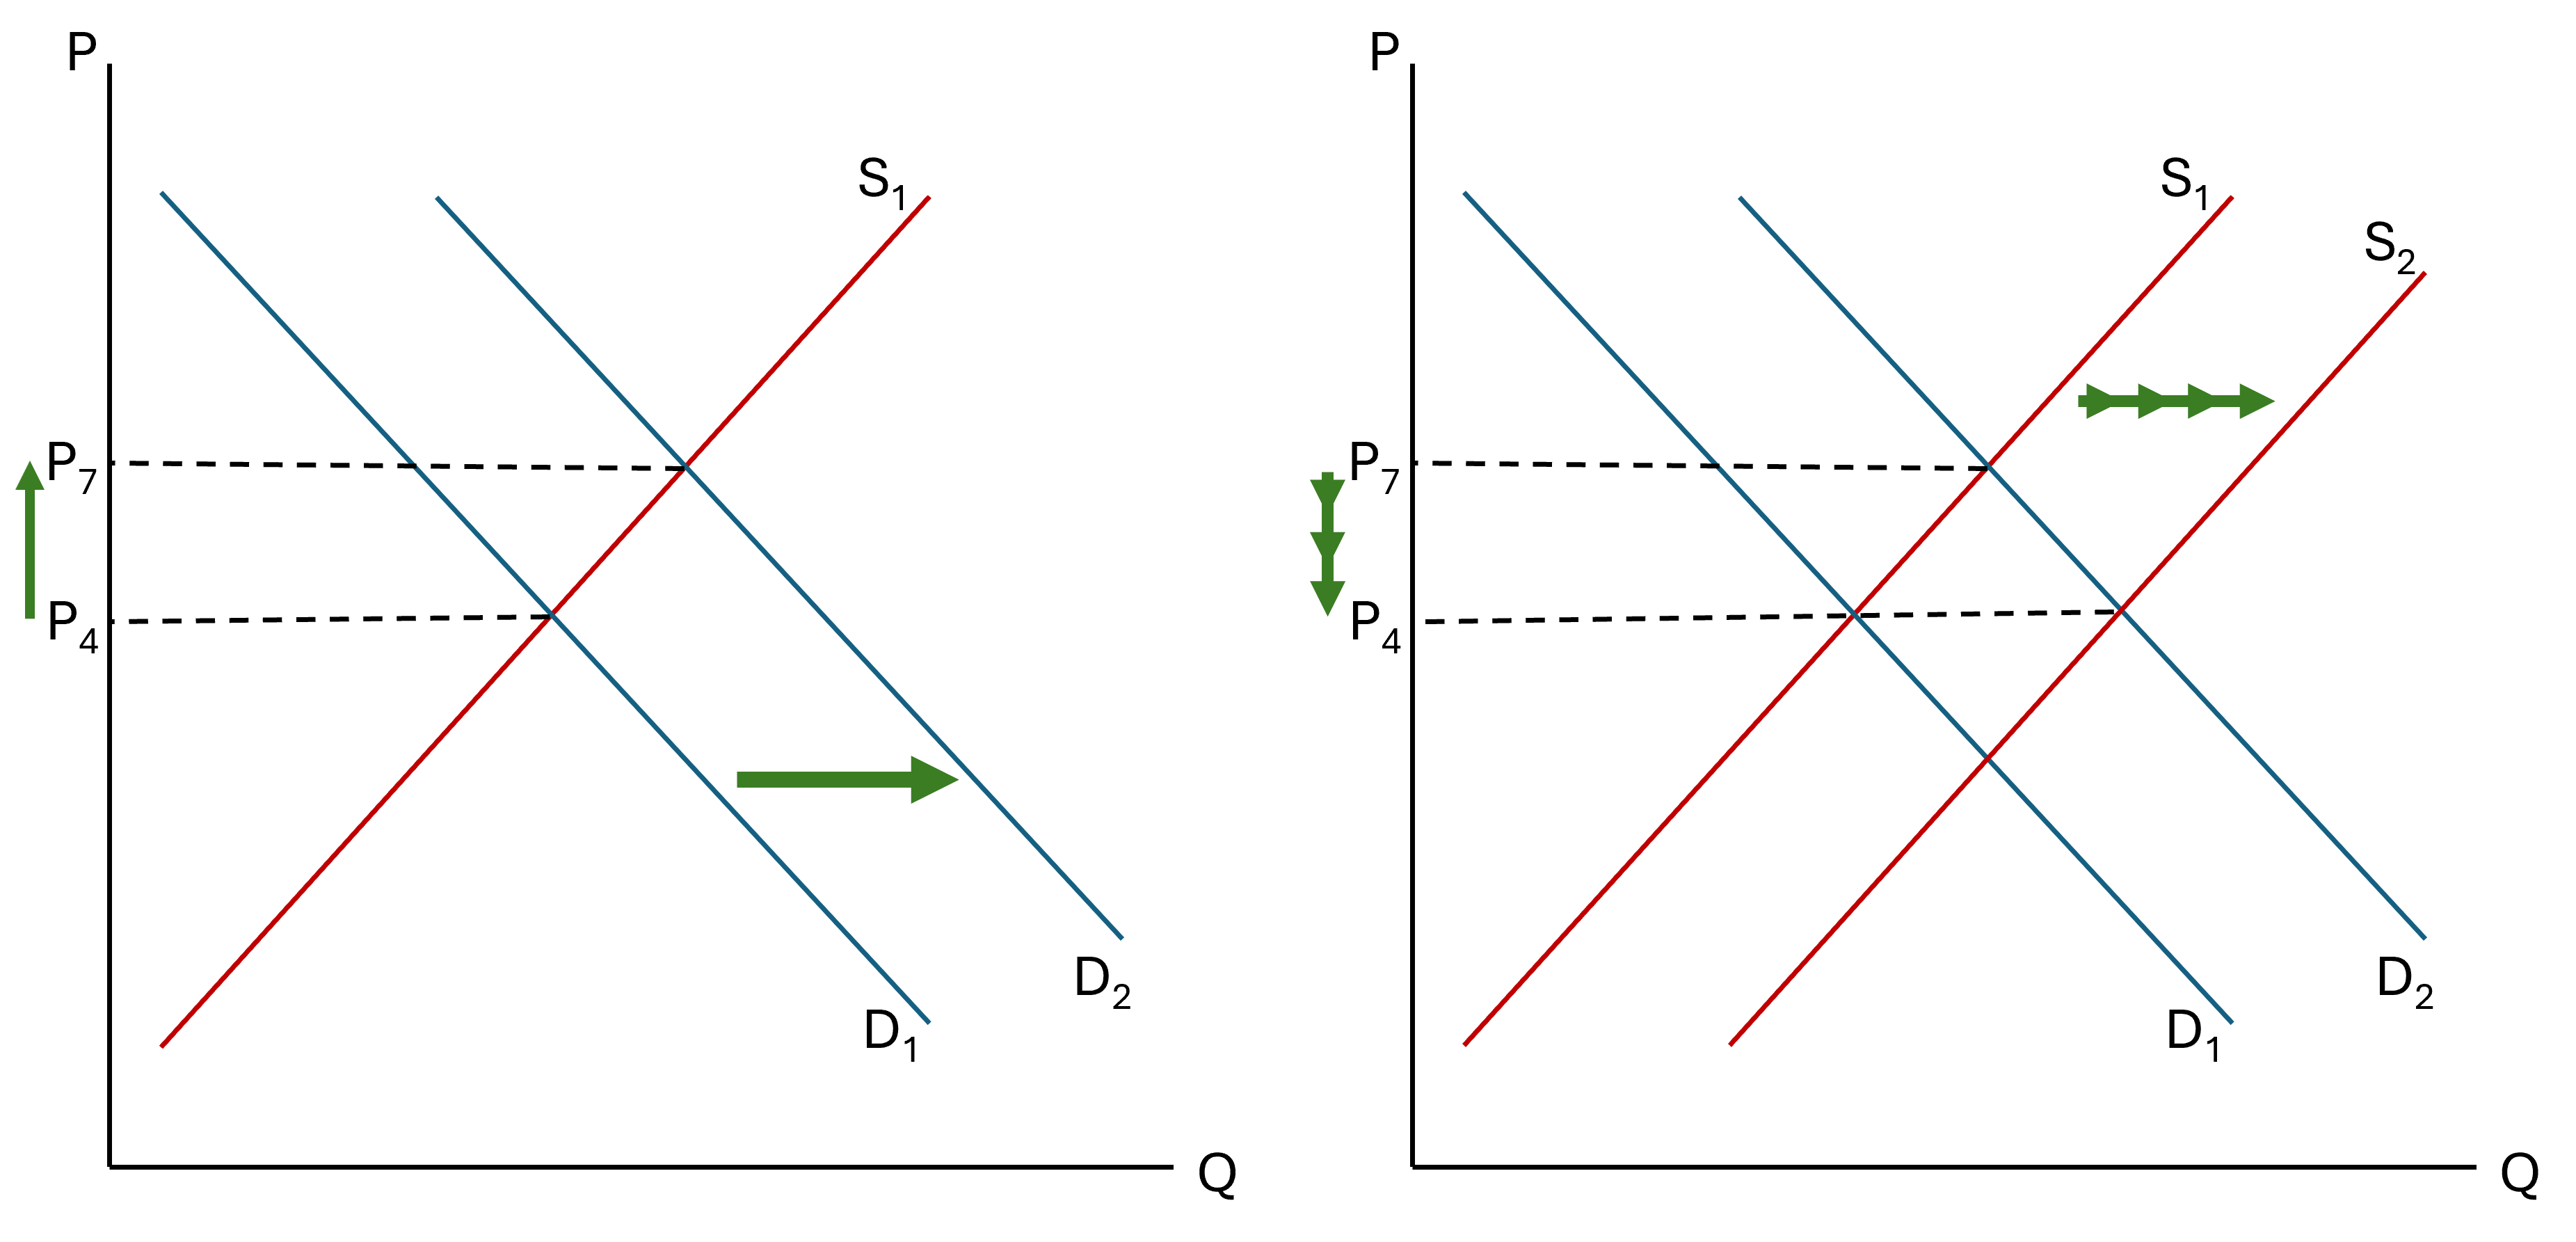
\includegraphics[width=\linewidth]{supply_increases.png}
\end{frame}

\end{document}

